\documentclass[12pt,a4paper,pdflatex]{article}
%%%%%%%%%%%%%%%%%%%%%%%%%%%%%%%%%%%%%%%%%%%%%%%%%%%%%%%%%%%%%%%%%%%%%%%%%%%%%%%%%%%%%%%%%%%%%%%%%%%%%%%%%%%%%%%%%%%%%%%%%%%%%%%%%%%%%%%%%%%%%%%%%%%%%%%%%%%%%%%%%%%%%%%%%%%%%%%%%%%%%%%%%%%%%%%%%%%%%%%%%%%%%%%%%%%%%%%%%%%%%%%%%%%%%%%%%%%%%%%%%%%%%%%%%%%%
\usepackage{amsmath}                                       % Símbolos matemáticos
\usepackage{amsthm}                                        % Símbolos matemáticos
\usepackage{amssymb}                                       % Símbolos matemáticos
\usepackage[round, longnamesfirst]{natbib}                 % Referencias bibliográficas
%\usepackage{cite}
%\usepackage{apacite} Permite utilizar el formato APA, revisar que version se esta utilizando.

\usepackage[spanish]{babel}
\usepackage[utf8]{inputenc}
\usepackage[center]{caption}
\usepackage{fancyhdr}
\usepackage{lscape}

%\usepackage{geometry}
\usepackage[top=4cm,bottom=2.5cm,left=3.5cm,right=2.5cm]{geometry}
%,footskip=0.25in
\usepackage{graphicx}                                      % Insertar figuras
\usepackage{epstopdf}
\usepackage{colortbl}                                      % Trabajar con colores
%\usepackage{hyperref}                                      % Vínculos y personalización del pdf
\usepackage{setspace}                                      % Espacios
\doublespacing
%\onehalfspace
%\singlespace
%\spacing{1.5}

\usepackage{rotating}                                      % Tablas horizontales \begin{sidewaystable}
\usepackage{enumitem}                                      % Listas personalizadas
\usepackage{booktabs}                                      % Comandos para tablas, e.g. \toprule
\usepackage{multirow}                                      % Para Tablas. Celdas formadas por múltiples filas
\usepackage{tabularx}
\usepackage{color}
\definecolor{darkred}{rgb}{0.5,0,0}
\definecolor{darkblue}{rgb}{0,0,0.5}
\usepackage[colorlinks,breaklinks,bookmarksnumbered,bookmarksopenlevel=2,unicode]{hyperref}               % Vínculos y personalización del pdf
\hypersetup{
  colorlinks,
  citecolor=darkred,
  linkcolor=darkred,
  urlcolor=darkblue,
	bookmarksopen=true, bookmarksopenlevel=3
	}

\usepackage{float}
\usepackage{lscape}
\usepackage[centerlast]{subfigure}
\usepackage{rotfloat}
\usepackage{caption}
\usepackage[section]{placeins}
\usepackage{bbm}
\usepackage{anysize}
\usepackage[T1]{fontenc}
\usepackage{titlesec}
\usepackage[scaled]{uarial}
\renewcommand*\familydefault{\sfdefault}

%%%%%%%%%%%%%%%%%%Formato del titulo
%\titleformat{\section}
%			[display]
% 			{\normalfont\huge\bfseries}
% 			{\thesection}{10pt}{\Huge}
%\titlespacing*{\chapter}{0pt}{50pt}{40pt}	

\titleformat{\section}[block]
{\normalfont\LARGE\filcenter}{\thesection}{1em}{}
%	{\normalfont{\thesection}}

\setcounter{MaxMatrixCols}{10}
%\bibliographystyle{BiblioStyle}
%\definecolor{darkred}{rgb}{0.5,0,0}
%\definecolor{darkblue}{rgb}{0,0,0.5}
%\hypersetup{
%  colorlinks,
%  citecolor=darkblue,
%  linkcolor=black,
%  urlcolor=darkblue,
%bookmarksopen=true, bookmarksopenlevel=3
%}
\captionsetup{format     = plain}
\captionsetup{labelsep   = period}
\captionsetup{labelfont  = {sc, bf}}
\captionsetup{textfont   = it}


%%%%%%%%%%%%%%%%%%% Títulos de figuras y cuadros
\usepackage{caption}
\captionsetup{format     = plain}
\captionsetup{labelsep   = period}
\captionsetup{labelfont  = {sc, bf}}
\captionsetup{textfont   = it}
%%%%%%%%%%%%%%%%%%%% Símbolos para las primeras notas al pie

%%%%%%%%%%%%%%%%%%%% Apéndices (macro \Apendice y comando \apendice)

%%%%%%%%%%%%%%%%%%%% Bibliografía

%%%%%%%%%%%%%%%%%%%%%%% Carpeta de gráficos

%%% Encabezados y pie de páginas and footers eliminate widows and orphan lines

\begin{document}
%\portada

\thispagestyle{empty}
\newpage
\begin{abstract}
Insertar abstract\\
\\
Palabras Claves:\\
Clasificación JEL:
\end{abstract}
\thispagestyle{empty}
\newpage

%%% Flushright

%%% Contenido
\tableofcontents
\thispagestyle{empty}
\newpage
\listoffigures
\thispagestyle{empty}
\newpage
\listoftables
\thispagestyle{empty}

\newpage
%\spacing{5}


\section{\underline{Introducción}}\label{sec1}
\pagestyle{fancy}
\fancyhf{}
\fancyhead[R]{\thepage}
\pagenumbering{roman}

\doublespacing

La revolucion digital es un proceso de creacion de nuevas tecnologias disruptivas. Estas tecnologias tienen la capacidad de transformarse continuamente, diversifcarse progresivamente e impulsar la productividad en todos los sectores e industrias.\\
Esta transformacion digital, principalmente dirigida por el internet, implica no solo la adaptación de nuevas tecnologias sino ademas, requiere que la economia se adapte a esta. La creacion de nuevas plataformas digitales son un ejemplo de como se ha reformulado la relacion entre los clientes, los trabajadores y los empleadores en la economia. A traves de estas plataformas se puede adquirir desde un producto para el hogar hasta un prestamo de consumo. Esto implica no solo una transformacion en los trabajos u oficios habituales de la economia, sino tambien, el replanteamiento completo de industrias como el comercio minorista, la industria editorial, y en un mundo no lejano, el sector bancario. \\
El comercio minorista refleja visiblemente la transformacion digital de una industria y que da origen a una nueva industria conocida como el comercio electronico o e-commerce.



La aparición de nuevas entidades o instituciones explican gran parte de esta revolución. \\
Las Fintech ofrecen servicios financieros a traves de plataformas digitales que las instituciones financieras como los bancos no pueden \\
La aparicion de las monedas digitales como el bitcoin representan una nueva forma de acumular riqueza o comprar bienes sin la necesidad de dinero fisico. \\
Por ultimo, la nueva forma de permutar productos a traves del comercio via internet conocido como e-commerce ,.... \\
Lo anterior ha despertado la preocupacion de los policy makers a como responder antes estas nuevas pertubaciones.

\newpage

%\spacing{}
\section{\underline{Revision de la literatura}}\label{sec2}
Los estudios clásicos del traspaso del tipo de cambio a nivel agregado encuentran un traspaso incompleto de corto y largo plazo \citep{burstein2014international, bussiere2013exchange}.

Por otro lado, la literatura reciente del traspaso pretende capturar los factores que están detrás este coeficiente incompleto, a través del uso de datos a nivel micro. Tal nivel de desagregación permite la identificación única de los productos a trabajar y establece diferencias específicas como el lugar de tienda vendida, el tipo de producto, si son productos importados o producidos localmente.

El primer factor que explica el traspaso incompleto del tipo de cambio son las rigideces de precios. Los modelos agregados macroeconómicos admiten la existencia de fricciones en el proceso de fijación de precios y estos explican la baja reacción de los precios ante choques agregados. Los costos de menú contabiliza el costo de optimizar continuamente los precios y ello deriva a que las empresas decidan sus precios en base a aquel que minimiza la pérdida. \textcolor{red}{Este párrafo está raro}

A nivel microeconómico, los modelos de costo de menú incorporan la existencia de ofertas o descuentos repentinos en la decisión de fijar precios (Kehoe y Nakamura, 2010; Guimaraes y Sheedy, 2011; Burstein y Hellwig, 2007). Las empresas están expuestas a dos situaciones, éstas pueden optimizar continuamente sus precios sujetos a los costos que envuelven esta decisión o cambian sus precios temporalmente (precios de oferta) a un bajo costo (Kehoe y Nakamura, 2010). En el modelo los precios de oferta, los agentes deciden ajustar sus precios temporalmente en vez de fijar por tiempo prolongados.

La poca rigidez de los precios a nivel micro explicada por la opción que tienen las firmas de cambiar precios temporalmente ayuda a entender un comportamiento más flexible de los precios a nivel micro a comparación del nivel agregado. Ello se debe a que los cambios de precios de oferta desagregados son transitorios (temporales) y no tienen ningún impacto sobre los cambios de precios a nivel agregado (Nakamura y Steinsson, 2013).

Por último, la lentitud del ajuste de precios puede estar relacionado con las fallas de coordinación que presentan las tiendas minoristas o las firmas al momento de tener la intención de ajustar precios. En Nakamura y Steinsson (2013) se ejemplifica una situación donde las firmas toman decisiones basadas en las acciones de las demás firmas. Al efectuarse un choque agregado, la empresa A no responderá a un ajuste de precios porque la empresa B no ha reaccionado todavía.

El segundo factor que explica el traspaso incompleto a nivel micro es el grado de competencia del sector y la calidad del producto (Gross y Schmitt 2000; Kim y otros, 2003). En Kim y otros (2003) se interpreta que a menor grado de competencia en un mercado, mayor será el traspaso de tipo de cambio; y contrario, a mayor grado de competencia, menor será el traspaso. El estudio compara el nivel de traspaso en dos mercados importadores de trigo, Japón y Corea. Además, un estudio aplicado para Perú encuentra los mismo resultados para el mercado de autos usados. El traspaso hacia los autos usados es menor cuando la estrechez del mercado aumenta; es decir, existe mayor competencia (Castellares, 2018).

Por otro lado, es posible admitir la existencia de una relación no lineal entre el grado de competencia y el nivel de traspaso (Gorodnichenko y Talavera, 2017). Se estima una relación de forma U invertida, donde a mayor competencia se encuentra un mayor traspaso pero hasta cierto umbral de número de firmas. Pasada las 4 firmas, el traspaso es menor a mayor competencia.

Adicionalmente, se estima utilizando datos desagregados que los precios reciben un menor impacto de las fluctuaciones cambiarias cuando se consideran bienes de mayor calidad (Auer y Chaney, 2009). En este modelo de Mussa y Rossen, se encuentra un traspaso heterogéneo e incompleto a nivel de industria.  Una depreciación del tipo de cambio del país importador produce dos efectos: una contracción en la oferta de cada variedad importada y la no importación de los productos de calidad más baja. Al disminuir la cantidad importada de bienes de calidad baja, se produce un cambio hacia un mayor consumo de bienes de calidad alta.

El tercer factor que explica el traspaso incompleto está negativamente correlacionado con los costos de búsqueda (Head, Kumar, and Lapham, 2010; Richards, Gómez, and Lee, 2014). Los retornos de búsqueda son mayores cuando se aplica para productos que son considerados caros o tienen un valor de compra alto. Es decir, los consumidores están más dispuestos a invertir un mayor tiempo comparando precios a productos como televisores o computadoras que en productos como un cepillo de dientes o unos auriculares (Gorodnichenko y Talavera, 2017). Una mayor intensidad de búsqueda puede generar una mayor presión de convergencia entre distintos vendedores e incluso países. En esta situación, en Gorodnichenko y Talavera (2017), se encuentra una relación no lineal entre traspaso y costo de búsqueda. \textcolor{red}{¿Cómo es esta relación no lineal?. Esto es clave. Se debe comentar estos efectos también cuando se expliquen los resultados de la tesis pues allí se distinguen items caros y baratos.}

El cuarto factor no estructural relaciona la flexibilidad de los precios a través de la frecuencia de cambios y duración con el nivel de traspaso (Gorodnichenko y Talavera, 2017; Cavallo, 2017 y 2018; Gopinath e Itskhoki, 2010). Desde un punto de vista micro, una forma de caracterizar las rigideces son a través de la frecuencia de cambios y la duración. Estudios de la escuela clásica con datos a nivel micro del Índice de Precios del consumidor (CPI) mostraban una frecuencia de cambios mensual del 21\% y una duración mediana de 4.3 meses (Bils y Klenow, 2004). Estudios más actualizados, encuentran que los precios de tiendas minoristas presentan una mayor frecuencia y menor duración debido a la aparición de un nuevo sector competitivo conocido como el comercio electrónico. Esta mayor flexibilidad se transmite en un mayor nivel de traspaso porque encuentra que un mayor cambio se refleja como mayor sensibilidad de respuesta ante choques agregados (Cavallo,2018).

La clasificación del producto tiene impacto sobre el grado de flexibilidad, por ejemplo, se tiene que los bienes durables presentan una flexibilidad menor que los producto perecibles (Nakamura y Steinsson, 2013).

Por último, un factor recientemente incorporado es el tiempo del inventario y su relación con el traspaso de tipo de cambio. Las tiendas minoristas suelen manejar productos que presentan problemas como los retrasos de envíos y los costos fijos por importar. Por tal motivo, la reacción óptima de estas tiendas es importar infrecuentemente y mantener inventarios; es decir, tener un almacenamiento de sus productos (Alessandria y otros, 2010).

En el documento de Alessandria y otros (2010) se modela que el precio de las tiendas minoristas depende del valor de un incremento adicional del stock de inventarios. Si el nivel de inventarios es muy alto, la firma decidirá bajar su precio por debajo del valor de tener una unidad adicional de inventario. De ocurrir un aumento de los precios importados y encontrarse en la situación donde sea alto el inventario, el traspaso será incompleto porque la tienda tendrá una mayor disposición de bajar precios con lo que hace el efecto de subida menor.

En Álvarez y otros (2018), se encuentra una relación negativa entre el número de días almacenado un producto y el precios óptimo a vender. La base de datos de la investigación utiliza datos micro de productos perecibles y encuentra que independientemente del nivel de tipo de cambio, los productores están dispuestos a aceptar un menor precio conforme aumenta el número de días almacenado. Intuitivamente, los vendedores tienen una mayor disposición a vender más rápido los productos más perecibles  lo que se traslada en un menor traspaso del tipo de cambio.

La revisión de literatura presentada resume las factores que explican un traspaso heterogéneo e incompleto dado la característica de la base de datos. A tal nivel de desagregación es posible identificar características específicas de los productos como su clasificación de la tienda, la clasificación de la calidad del producto, el grado de competencia del mercado, la flexibilidad de cambio de precios o lo contrario, la rigidez. Esto permite tener una comprensión más clara de cómo diversos factores pueden influenciar la reacción de un determinado precio ante un mismo choque como es el tipo de cambio. A diferencia de los estudios a nivel agregado que no permite capturar tal grado de heterogeneidad.

\newpage
\begin{table}[!h]
\centering
\caption{Resumen de revisión de Literatura}\label{cor1}
\scalebox{0.7}{
\begin{tabular}{p{2.5cm}m{3em}m{3.5cm}m{3cm}m{2.5cm}m{3cm}}
  \hline
  % after \\: \hline or \cline{col1-col2} \cline{col3-col4} ...
  \textbf{Autor(es)} & \textbf{Países} & \textbf{Variables relevantes} & \textbf{Controles} & \textbf{Estimación} & \textbf{Datos y muestra} \\
  \hline
  \hline
  Kochen y Sámano(2016)& México & Variación del precio de los productos.Variación acumulada del tipo de cambio entre cambio de precios. & Precio internacional de los commodities. Precio del productor de electricidad Salarios promedio diarios. Cambios en los precios por ofertas. & Con controles: 0.0073\% & Micro datos del CPI. Mensual 2011-2016\\
 \hline
  Antoniades y Zaniboni(2016)& Emiratos Árabes Unidos & Variación promedio bimensual de los precios. Variación del tipo de cambio
en la misma frecuencia de los precios. & Proxy de cambios de costo marginal: Cambios en los precios extranjeros. Proxy de cambios en demanda doméstica: Valor de las ventas totales de cada producto & Largo plazo (1 año): 20\% & Precios escaneados de bienes
de rápido consumo de tiendas minoristas. Mensual-Bimensual 2006-2010\\
 \hline
  Aron et al(2014) & Sudáfrica & Variación del precio del bien(6 meses de diferencia). Variacion del tipo de cambio de 6 meses hasta 2 años & Proxy de Costos extranjeros. Proxy de Costos de labor doméstico & PT Largo plazo. Alimentos:20\%.Vestimenta y medicionas: 10\% & Bienes unicos
del CPI. Mensual 2001-2007\\
 \hline
  Castellares(2017)& Perú & Variación del precio del auto(Precio de su ultima aparición contra la primera). Variación del tipo de
cambio nominal & Proxy de calidad: tamaño del precio promedio del auto. Proxy de demanda: búsqueda en Google trends de autos usados. Proxy de competencia: los días que demoro en vender el auto & Sin controles:
27 \% Control de calidad: 35.5 \% Control de competencia: 66.4 \% & Precios de autos usados
publicados en El Comercio Diaria. Semanal 2014-2016.\\
  \hline
  Álvarez et al (2016)& Turquia & Variación diaria de los precios del productor importado. Variación del tipo de cambio en la frecuencia de los precios & Inflación diaria de los productos agrícolas locales. Periodo de almacenamiento del producto & Traspaso completo inmediato a bienes importados denominados en euro. Traspaso incompleto y rapido a bienes importados denominados en franco suizo. & \\
  \hline
\end{tabular}
\label{table:1}
}
\end{table}

\newpage
\begin{table}[!h]
\caption{Resumen de revisión de Literatura}\label{cor1}
\centering
\scalebox{0.7}{
\begin{tabular}{p{2.5cm}m{3em}m{3.5cm}m{3cm}m{2.5cm}m{3cm}}
  \hline
  % after \\: \hline or \cline{col1-col2} \cline{col3-col4} ...
  \textbf{Autor(es)} & \textbf{Países} & \textbf{Variables relevantes} & \textbf{Controles} & \textbf{Estimación} & \textbf{Datos y muestra} \\
  \hline
  \hline
  Bonadio, Fischer y Sauré(2016)& Suiza & Unidades de valor de las importaciones. Cuantifica el impacto de un gran shock cambiario
a través de dummies & Dummies mensuales. Dummies diarios & Traspaso completo inmediato a bienes importados denominados en euro. Traspaso incompleto y rapido a bienes importados denominados en franco suizo. & Datos de comercio del Swiss Customs Administration. Diaria 2012-2015\\
  \hline
  Cavallo(2018)& Estados Unidos & Variación del indice de precios a nivel de sector. Variación del tipo de cambio nominal& - & Corto plazo(2 trimestres): 16\% Largo plazo(2 años): 31\% & Indice de precios de productos de tiendas minoristas computados por PriceStats. Trimestral 2008-2017\\
  \hline
  Gorodnichenko y Talavera(2017)& Canadá y Estados Unidos & Nivel de los precios relativos Nivel del tipo de cambio nominal & Efectos fijos por producto & Largo plazo: Sin controles: 76.5\% Con controles:67\% & Precios de productos de tiendas minoristas obtenidos de páginas web comparadoras de precios (PWC)Semanal 2008-2013 \\
  \hline
  Boivin et al(2011) & Canadá y Estados Unidos & Diferencia del nuevo precio con respecto al último precio registrado. Variación del tipo de cambio acumulado& Dummy de meses. Número de meses desde la publicación del libro i.& Precios de libros obtenidos en Estados Unidos: Pagina web Amazon y Barnes and Noble’s. Canada: Pagina web de Amazon y Chapters. & Mediano Plazo: No encuentra una relación del tipo de cambio hacia los precios relativos. Tres días a la semana 2008-2009 \\
  \hline
  Gorodnichenko y Talavera(2017)& Canadá y Estados Unidos & Nivel de los precios relativos Nivel del tipo de cambio nominal & Efectos fijos por producto & Largo plazo: Sin controles: 76.5\% Con controles:67\% & Precios de productos de tiendas minoristas obtenidos de páginas web comparadoras de precios (PWC)Semanal 2008-2013 \\
  \hline

\end{tabular}
\label{table:1}
}
\end{table}

\clearpage
\section{\underline{Descripción de los datos}}\label{sec4}

El estudio utiliza datos recolectados de la plataforma del canal de venta \textit{online} de \href{https://www.falabella.com.pe/falabella-pe/}{Saga Falabella} que contiene información de los productos y los precios listado por la tienda minorista. \\
El proceso de captura de los datos se realiza diariamente y se ejecuta a través de un programa codificado en el lenguaje R. El programa se encarga de la identificación de las categorías establecidas de la página web y depura aquellas categorías que no pertenecen al conjunto de productos considerados como electrónicos. El resultado de esta primera etapa determina el número de las categorías a trabajar, resumidas en el Cuadro \ref{cor1}. \\

%\caption{Tabla1:Descripción de las categorias de productos}\label{cor1}
%\centering
%\scalebox{0.7}{
%\begin{center}

\begin{table}[h!]
\caption{Descripción de las categorías de productos}\label{cor1}
\centering
\begin{tabular}{lcrccrcc}
\toprule
\multirow{2}{*}{Categoría}& \multicolumn{3}{c}{Número de}     & \multicolumn{3}{c}{Número de}          & \multirow{2}{*}{B / A} \\
                          & \multicolumn{3}{c}{productos (A)} & \multicolumn{3}{c}{observs. (B)}  &   \\
\midrule
Audio                     & &200    &                         &  &  87 628 & & 438\\
Computadores              & &162    &                         &  &  68 942 & & 426\\
Electrodomésticos         & &390    &                         &  & 174 357 & & 447\\
Electrohogar              & & 17    &                         &  &   7 427 & & 437\\
Fotografía                & & 69    &                         &  &  31 144 & & 451\\
\addlinespace
Linea blanca              & &360    &                         &  & 166 528 & & 463\\
Teléfonos                 & & 39    &                         &  &  14 857 & & 381\\
Televisores               & & 33    &                         &  &  12 331 & & 374\\
\midrule
Total                     & &1 270  &                         & &  563 214 & & \\
\bottomrule
\end{tabular}
%\caption{Descripción de las categorías de productos}
\label{table:1}
\end{table}


El siguiente paso consiste en recorrer los ocho enlaces de internet, uno para cada categoría. En cada enlace se realiza la extracción de la información requerida para cada producto. La información contiene el nombre del producto o descripción, la marca, el rating o puntaje de calidad y tres precios. El primer precio se denomina como precio normal e indica el valor del producto que se tranza por el canal físico. Es decir, es el precio que se paga por el producto cuando se compra de manera tradicional, yendo a la propia tienda.

El segundo precio se denomina precio de internet indica el valor del producto que se tranza por el canal virtual. Es decir, es el precio que se paga cuando se realiza la compra a través de la página web. Por último, el tercer precio capturado es el precio asociado a la membresía de la tarjeta de crédito de Saga.

Los datos recolectados diariamente se apilan en una gran base, y luego de un proceso de limpieza, se transforma en un panel donde la unidad de análisis es a nivel de producto.\\
El periodo de recolección inicia el 19 de setiembre del 2016 hasta la última actualización de los datos, el 30 de abril del 2019. Debido a que los precios se descargan todos los días, esta base de productos electrónicos se caracteriza por su alta frecuencia y la desagregación de los datos a nivel micro.\\
El cuadro \ref{cor2}, resume el número de observaciones para cada clasificación de precios. El número de observaciones para la variable precio de internet y precio normal son iguales; en cambio, las observaciones del precio miembro son la tercera parte. Esto se explica porque los descuentos utilizando tarjetas de crédito se realizan en algunas épocas del año. \\

\begin{table}[h!]
\caption{Número de observaciones y precios}\label{cor2}
\centering
\begin{tabular}{lr}
\hline
Tipo de precio &  N de observaciones\\ \hline
Precio normal & 563 214 \\
Precio de internet & 563 214 \\
Precio miembro & \textcolor{red}{¿?}\\
\hline
\end{tabular}
\label{table:1}
\end{table}

Al final se recolectan 563214 precios y 1270 bienes o productos. Esta base de datos considera productos clasificados en ocho categorías: computadoras (162 productos), electrodomésticos (390 productos), electro-hogar (17 productos), fotografía (69 productos), línea blanca (360 productos), teléfonos (39 productos), televisores (33 productos) y audio (200 productos). \\
La base de datos descrita presenta diversas propiedades que permiten realizar el estudio del traspaso de tipo de cambio. La primera característica importante es el sector central al que pertenecen los productos. En el cuadro \ref{cor1}, se puede observar que todos los productos a analizar pertenecen al grupo de electrónicos, este grupo de bienes son los que presentan una mayor participación de ventas junto con ropa o vestimenta dentro del comercio electrónico (\textcolor{red}{alguna fuente para esto?}). Si bien no representa todo el comercio electrónico, este sería un paso importante para caracterizar específicamente este sector tan relevante.

Asimismo, los precios son recolectados de la página web Saga Falabella, tienda que representa alrededor del 50\% del mercado minorista (\textcolor{red}{fuente?}). En base a esto, los resultados encontrados permiten realizar una generalización para el resto del sector de electrónicos; debido a que, un comportamiento de los precios pertenecientes a esta tienda puede darnos una idea de cómo se comporta el resto del sector.

La segunda característica a resaltar es la duración del periodo de estudio. Esta base de datos considera información de dos años y medio, lo que permite tener un horizonte de análisis superior a muchos otros estudios que tiene un año de recolección.

La tercera característica es el nivel de desagregación de la base de datos, eso significa que cada producto es perfectamente identificable a nivel de bien y adicional a esto la  frecuencia de los datos de cada bien es alta. Esto implica que es posible diferenciar entre dos productos exactamente iguales, de la misma marca, mismo modelo pero lo único que los diferencia es el color. Adicionalmente, la desagregación permite también capturar efectos heterogéneos de las estimaciones por categorías propias de los bienes.

Por último, los tres tipos de precios permiten realizar un estudio adicional que es el análisis del comportamiento de los precios de internet contra los precios de tienda física. Esto es relevante con la finalidad de corroborar o diferir de los hechos estilizados encontrados en otros países como Estados Unidos y Canadá. La literatura describe que los precios de internet deben ser más flexibles debido a que no presentan las mismas rigideces que los precios en el mercado físico como los costes de menú. Por tal motivo, en esta sección se realiza tal caracterización del comportamiento de los precios.

\clearpage

\textbf{Caracterización de la base de datos}

El proceso de construcción y limpieza de la base de datos incluía una depuración de bienes que no contengan información de más de 240 días. Esto permite eliminar bienes que tienen apariciones repentinas que no permiten capturar el comportamiento de los precios en un largo periodo de tiempo sino que solo por pequeñas ventanas de tiempo.

En la figura 1 se muestra el histograma del número de observaciones por cada bien, y se detalla que los productos tienen por lo menos 240 observaciones, la mayor parte está concentrado en el rango de 240 y 360 observaciones. Asimismo, existen productos que tienen un periodo de aparición más prolongado con observaciones superiores a 400 y la máxima con 511 observaciones. Existe una distribución con poca varibilidad de las observaciones por producto y detalla que la base es un panel no balanceado.
\begin{figure}[!ht]
\centering
 \caption{Histograma del número de observaciones por bien}
  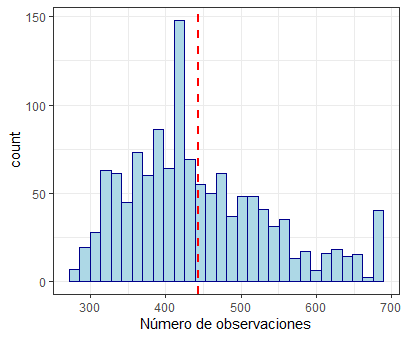
\includegraphics[scale=1.0]{observaciones_producto.png}
  \label{fig:Histograma del número de observaciones por bien}
\end{figure}

\clearpage
\textbf{Clasificación de los bienes} \\

En la siguiente figura se puede observar la densidad del número de observaciones por la clasificación de cada producto. Esta figura muestra que a través de cada categoría los bienes independiente de su clasificación tienen una concentración de observaciones de 350 a 450. Esto permite ver la uniformidad de la base de datos y también encontrar diferencias entre cada categoría. Por ejemplo, las categorías como línea blanca, fotografía y electrohogar presentan bienes que tienen el número máximo de observaciones, alrededor de 670.  Por otro lado, televisores y teléfonos son categorías cuyos productos tienen un menor número de apariciones en los dos años y medio de recolección, sus datos tienen como máximo 500 observaciones. Aunque en general, entre categorías presentan una variabilidad razonable.

\begin{figure}[!ht]
\centering
 \caption{Gráfico de densidad del número de observaciones por categorías}
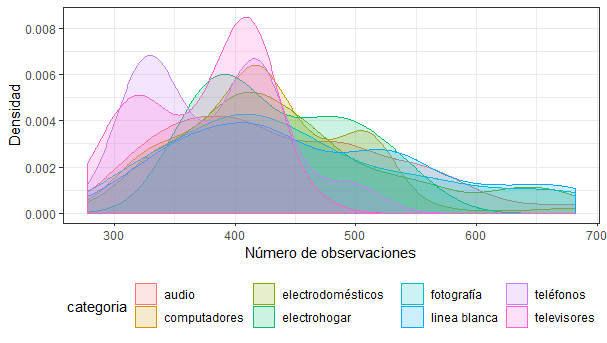
\includegraphics[scale=1.0]{observaciones_categoria.png}
  \label{fig:Gráfico de densidad del número de observaciones por categorías}
\end{figure}

\clearpage
\textbf{Porcentaje de cambios de la vida de un bien} \\
Este indicador se calcula identificando el número de cambio de precios que cada producto ha tenido durante su aparición en la base de datos. El ratio de este indicador tiene en su numerador el número de cambios totales de un bien y en el denominador el número de observaciones totales por producto y multiplicado por 100, obtenemos qué parte de la aparición de un bien ha cambiado.

El indicador permite cuantificar el grado de flexibilidad de los precios de internet con el objetivo de comprobar relación entre flexibilidad y mayor sensibilidad de reacción ante los choque macroeconómicos que resalta la literatura (Cavallo, 2017). Por lo tanto, se espera que esta flexibilidad se refleje en un mayor traspaso del tipo de cambio. Por otro lado, en Cavallo (2018), se describe que los precios de internet deben tener una mayor flexibilidad que los precios de tienda física debido a que no tienen presenten las mismas fricciones físicas y el costo de actualizar precios es casi nulo.

En ese sentido, con la finalidad de mostrar que los precios de internet presentan una mayor flexibilidad, se procede a comparar gráficamente el indicador de porcentaje de cambios para ambos tipos de bienes.

En la figura 4, se muestra el histograma del indicador elaborado para los precios de tienda física y se ve la gran diferencia con la figura 3. El porcentaje de cambios está prácticamente centrada en cero donde gran parte de los datos se encuentran. Es decir, los precios de tienda física no cambian en realidad y se encuentra un valor máximo de 5\%. Por lo tanto, se puede concluir que los precios de internet presentan una mayor flexibilidad.

\begin{figure}[!ht]
\centering
 \caption{Histograma del porcentaje de cambios: Precio online}
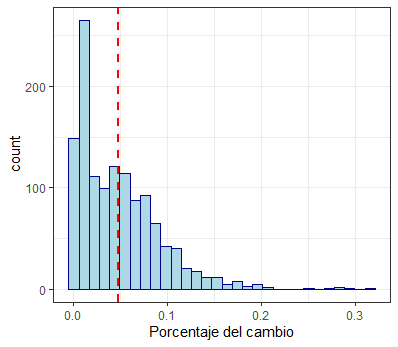
\includegraphics[scale=1.0]{cambio_producto_internet.png}
  \label{fig:Histograma del porcentaje de cambios: Precio online}
\end{figure}


\begin{figure}[!ht]
\centering
 \caption{Histograma del porcentaje de cambios: Precio offline}
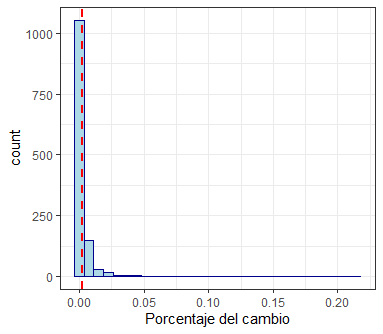
\includegraphics[scale=1.0]{cambio_producto_normal.png}
  \label{fig:Histograma del porcentaje de cambios: Precio offline}
\end{figure}

\clearpage

\textbf{Frecuencia de cambios diaria}\\
El indicador de porcentaje de cambios del bien muestra mayor flexibilidad de los precios de internet comparado con los precios de tienda física. Este resultado se mantiene utilizando otra serie conocida como el cambio de precios diario. Este se construye identificando las fechas del periodo de estudio; y por cada día, se calcula el número de bienes que han cambiado entre el número de bienes que se registraron.

En la figura 5 se observa el porcentaje de bienes que han cambiado precios para la base de datos y en promedio el 4\% de los datos cambian diariamente. Se observa que existen fechas en donde el porcentaje de cambios se incrementa y fechas donde toma valores bajos. Dentro de los valores picos el único patrón que se ha encontrado es un incremento del cambio de precios en noviembre para los tres años de la base.

De la misma forma que el análisis anterior, no se puede decir en absoluto que los precios de internet cambian en mayor cantidad pero si se puede realizar una comparación con los precios físicos. La figura 6 muestra que los precios físicos reflejan el comportamiento de cambios de la figura 4, existen días donde ningún ha cambiado precios y cuando se presenta el cambio no muchos producto ajustan sus precios. En este caso el porcentaje máximo de bienes que han cambiado en un dia es de 3.00 \%, mientras que los precios de internet llegan un valor máximo de 45\% lo que demuestra la mayor flexibilidad relativa.



\begin{figure}[!ht]
\centering
 \caption{Frecuencia de cambios por día: Precio online}
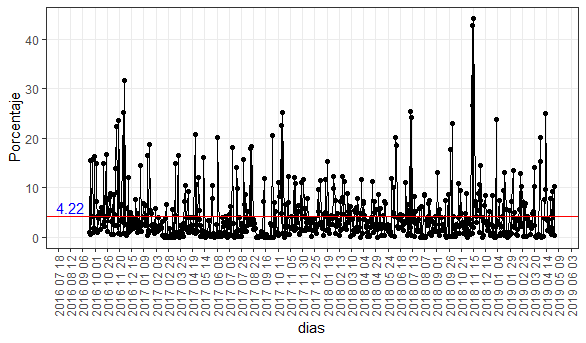
\includegraphics[scale=0.8]{frecuencia_dias_internet.png}
  \label{fig:Frecuencia de cambios por día: Precio online}
\end{figure}


\begin{figure}[!ht]
\centering
 \caption{Frecuencia de cambios por día: Precio offline}
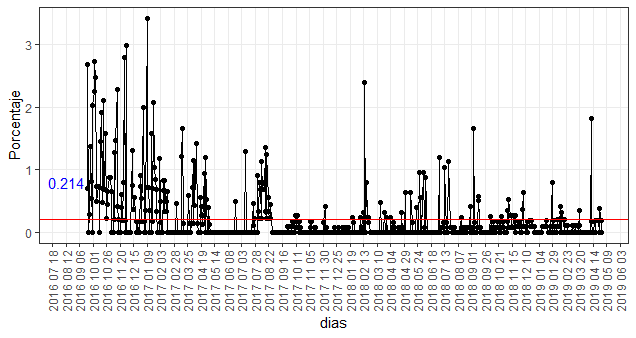
\includegraphics[scale=0.8]{frecuencia_dias_normal.png}
  \label{fig:Frecuencia de cambios por día: Precio offline}
\end{figure}

\clearpage

\textbf{Tamaño del cambio promedio por día} \\

La frecuencia de cambio de precios es mayor para los precios que se transan en el comercio electrónico en comparación de los precios de tienda física. Esto puede implicar otras propiedades de los precios. El efecto selección muestra que los precios que se caracterizan por ser no flexibles; es decir, tener un tiempo mayor tiempo sin actualizarse presentarán un tamaño de cambio muy fuerte. Para los precios que suelen actualizarse constantemente estos tamaños de cambio son pequeños porque el precio definido en un periodo está muy cerca del precio óptimo.

La figura 7 y 8 muestran en tamaño del cambio diario para los precios de internet y físico. Esta serie se calcula tomando el promedio del porcentaje del tamaño de cambio de precios por dia a lo largo del periodo de estudio. Comparando el promedio del tamaño del cambio diario, ambas series presentan el mismo valor. Sin embargo, es notable comparar que para el primer año de estudio, los precios de internet presentaban un mayor cambio. Oscilaban entre 10\% y 80 \% mientras los precios de internet entre 10\% y 50\%

\begin{figure}[!ht]
\centering
 \caption{Tamaño del cambio promedio por d\'ia: Precio online}
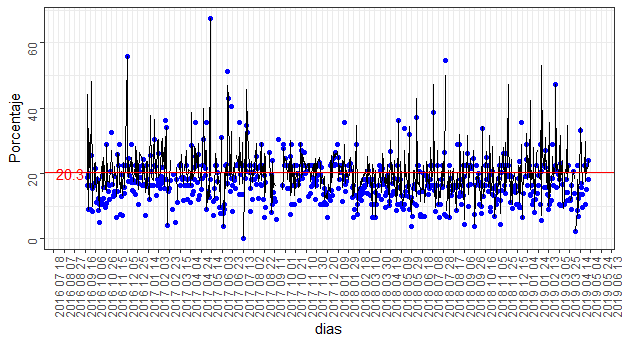
\includegraphics[scale=1.0]{tamano_cambio_promedio_internet.png}
  \label{fig:Tamaño del cambio promedio por d\'ia: Precio online}
\end{figure}


\begin{figure}[!ht]
\centering
 \caption{Tamaño del cambio promedio por d\'ia: Precio offline}
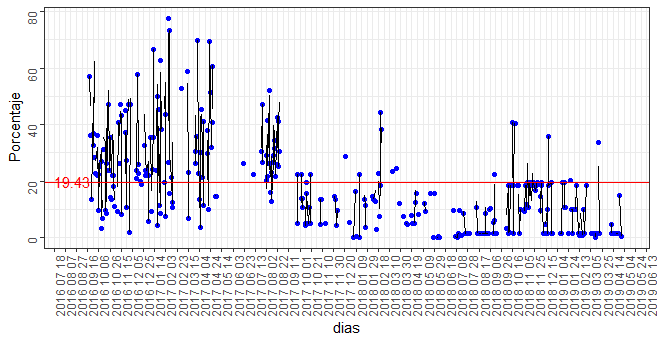
\includegraphics[scale=1.0]{tamano_cambio_promedio_normal.png}
  \label{fig:Tamaño del cambio promedio por d\'ia: Precio offline}
\end{figure}


\clearpage

%%%%%%%%%%%%%%%%%%%%%%%%%%%%%%%%%%%%%%%%%%%%%%%%%%%%%%%%%%%%%%%%%%%%%%%%%%%%%%%%%%%%%%%
\section{\underline{Marco Teórico}}\label{sec3}

El traspaso del tipo de cambio (ERPT) mide el nivel de reacción de los precios ante variaciones del tipo de cambio nominal para un determinado país. (Gopinath y Burstein, 2013) \\
La magnitud de respuesta de los precios en una economía puede ser heterogénea de acuerdo al tipo de precio a analizar. Estos se diferencian dependiendo del nivel en donde se determinen y en relación a estos niveles se logra identificar tres tipos: los precios de los consumidores o precios al por menor, los precios de los productores o precios al por mayor y los precios de las importaciones al por mayor.\\
En un estudio de Miller (2003), se describe que cada uno de los precios es vulnerable a las distintas perturbaciones que recibe la economía y el efecto de los choques puede ser trasladado de un nivel a otro o caso contrario, el efecto completo lo asume un determinado nivel de precios.  En este contexto, gran parte del grado del traspaso hacia cada precio se explica por la disposición de sacrificar márgenes de ganancias.\\
La interrelación de los precios permite entender la dinámica de un choque cambiario sobre estos. El texto de Gopinath y Burstein (2013) deriva un modelo económico que muestra las variables o fuerzas que determinan el comportamiento de los precios de los consumidores en relación a los precios de las importaciones. Los cambios del precio del consumidor están explicados por los cambios en los precios de los servicios de distribución y estos se refieren a los costos que asume la tienda minorista al ofrecer sus servicios locales, también por las variaciones del margen de la tienda minorista y por último, por los cambios del precio de las importaciones. El impacto de una depreciación cambiaria sobre los precios minoristas se explica por dos canales: el aumento del precio de las importaciones y la disminución del margen.\\
Los estudios presentados tienen en común la consideración de factores microeconómicos que relacionan los precios del consumidor con el tipo de cambio. El estudio del traspaso hacia los precios se ha enfocado en el estudio a nivel agregado. Sin embargo, existe otra variante que busca entender esta relación con el uso de datos a nivel desagregado o granular. Asimismo, se enfatiza el estudio del comportamiento de los precios de los consumidores o precios al por menor. \\
El traspaso captura la relación entre las dos variables enfatizadas: precios y tipo de cambio. En ese sentido, con la finalidad de caracterizar esta relación se analiza el traspaso desde tres aspectos. \\
Primero, la magnitud del coeficiente del traspaso permite cuantificar el nivel de respuesta de los precios atribuido a la variación de tipo de cambio. \\
En la mayoría de los estudios empíricos de traspaso se estiman variantes de la siguiente ecuación:
\begin{equation}
  \Delta P_{t} = \alpha_{0} +\alpha_{1}P_{t-1} +\alpha_{2}\Delta ER_{t}
\end{equation}

Donde $P_{t}$ es el precio en el periodo $t$ y $ER_{t}$ es tipo de cambio nominal en tiempo $t$. Asumiendo que un choque cambiario exogeno golpea sobre los precios, la ecuación anterior se puede expresar de la siguiente forma.
\begin{equation}
  \Delta P_{t} = \alpha_{0} +\alpha_{1}P_{t-1} +\alpha_{2}\delta
\end{equation}
El impacto se puede diferenciar por el tiempo de reacción de los precios como consecuencia del choque. La reacción inmediata al cambio del tipo de cambio se le denomina traspaso de corto plazo y la magnitud final cuando el precio alcanza su equilibrio luego del choque se le denomina traspaso de largo plazo. \\
Reescribiendo la ecuación $(2)$, se puede despejar el precio en función de su información pasada y el choque de tipo de cambio.
 $$P_{t}- P_{t-1} = \alpha_{0} +\alpha_{1}P_{t-1} +\alpha_{2}\delta$$
\begin{equation}
 P_{t} = \alpha_{0} + (1+\alpha_{1})P_{t-1} + \alpha_{2}\delta \\
 \end{equation}
 El precio expresado en su nuevo nivel de equilibrio se muestra en la ecuación $(4)$, y despejando podemos obtener el nuevo precio en función del choque cambiario.
 \begin{equation}
 \overline{P} =  \alpha_{0} + (1+\alpha_{1})\overline{P}+ \alpha_{2}\delta
\end{equation}
Donde $\alpha_{1}<0$ y un aumento del tipo de cambio en $\delta \%$ determinan el nuevo precio de equilibrio:
$$\overline{P} = \frac{-1}{\alpha_{1}}(\alpha_{0}+\alpha_{2}\delta)$$

De la ecuación$(1)$, el coeficiente $\alpha_{2}$ captura el traspaso del tipo de cambio en el corto plazo. Este coeficiente muestra el impacto directo y es explicito en la ecuación. Para poder obtener el coeficiente del traspaso de largo plazo, es necesario obtener el precio previo al choque y comparar con el nuevo precio de equilibrio \\
Donde $\overline{P'}$ representa el precio de equilibrio previo al choque, y tiene la siguiente forma.
\begin{equation}
 \overline{P'} = \alpha_{0} + (1+\alpha_{1})\overline{P'}
\end{equation}
$$\overline{P'} = \frac{-\alpha_{0}}{\alpha_{1}}$$

Se resta el precio de equilibrio luego del impacto $P$ y el precio de equilibrio antes del impacto $P'$ y el coeficiente que multiplica el cambio porcentual del tipo de cambio mide el traspaso del tipo de cambio.
\begin{equation}
 \overline{P} = \overline{P'} - \frac{\alpha_{2}}{\alpha_{1}}\delta
\end{equation}
$$\overline{P} - \overline{P'} = -\frac{\alpha_{2}}{\alpha_{1}}\delta$$

Asimismo, la proporción del cambio del tipo de cambio hacia los precios puede tomar valores desde 0 hasta 1. Si los precios reaccionan en la misma magnitud a la variación del tipo de cambio, el traspaso se le denomina completo. Por el contrario, si los precios reaccionan en una menor proporción se le denomina traspaso incompleto. \\

Segundo, la ecuacion $(1)$ caracteriza el traspaso como una relación lineal y simétrica. La simetria refiere a que un aumento de $\delta \%$ del tipo de cambio (depreciación) tiene el mismo impacto que una disminución (apreciación)y la linealidad refiere a que grandes devaluaciones o apreciaciones cambiarios tiene un impacto mayor sobre los precios que una pequeño movimiento del tipo de cambio. La ecuación se puede modificar de tal manera que se pueden incluir las asimetrias y no linealidades en el traspaso del tipo de cambio. En la literatura del traspaso a nivel agregado para el Perú, se ha encontrado la presencia de estos fenomenos y es interensante analizar esto a nivel micro.
Incluyendo asimetrías en la ecuación anterior, se reemplaza $\alpha_{2}\Delta ER_{t}$ por:
\begin{equation}
  \Delta P_{t} = \alpha_{0} +\alpha_{1}P_{t-1} +\alpha_{2A}A\Delta ER_{t} + \alpha_{2D}D\Delta ER_{t}
\end{equation}
Donde $A$ y $D$ se activan cuando se aprecia o se deprecia el tipo de cambio respectivamente. La literatura encuentra que las asimetrías se pueden explicar particularmente porque los precios presentan una mayor rigidez hacia bajo y las cantidades presentan mayores rigideces hacia arriba(Bussiere, 2007) \\
En el texto de Peltzman(2002) se resume la idea de que los precios suben mucho más rápido que cuando disminuyen, idea que puede cumplir a nivel micro y que explicaría la asimetria a este nivel. \\
Asimismo, se puede incluir el supuesto de no linealidad en la ecuación anterior:
\begin{equation}
  \Delta P_{t} = \alpha_{0} +\alpha_{1}P_{t-1} +\alpha_{2L}L\Delta ER_{t} + \alpha_{2S}S\Delta ER_{t}
\end{equation}
Donde $L$ se activa cuando ocurre un cambio del tipo de cambio superior a un umbral $\overline{\delta}$ y contrario, $S$ se activa cuando ocurre un cambio del tipo de cambio inferior al umbral $\overline{\delta}$.

Por ultimo, la velocidad de ajuste del traspaso mide el tiempo que le toma a los precios en reaccionar completamente al choque del tipo de cambio. \\

\clearpage
%%%%%%%%%%%%%%%%%%%%%%%%%%%%%%%%%%%%%%%%%%%%%%%%%%%%%%%%%%%%%%%%%%%%%%%%%%%%%%%%%%%%%%%%%%%%
\section{\underline{Metodología}}\label{sec3}
La finalidad de la presente investigación es encontrar una relación entre los nuevos precios conocidos como precios de internet y las fluctuaciones del tipo de cambio. Además, la literatura ha demostrado que a tal nivel de desagregación el traspaso hacia los precios es incompleto y el nivel depende de las características propias del bien.

En ese sentido, se plantea la metodología propuesta en Gopinath y Itskhoki (2010) denominada el Traspaso de Larga Vida (Life-Long PassThrough). Esta metodología no estructural documenta la relación del nivel del traspaso de los bienes con un factor que caracterice el comportamiento de los precios. Este enfoque estima el traspaso del tipo de cambio sobre la vida de un precio en la base de datos de estudio. Es decir, para cada bien se estima el efecto de la variación del tipo de cambio acumulado sobre la variación acumulada del precio desde su nacimiento hasta que se registra un nuevo precio.

En la figura 9 se muestra un ejemplo hipotético de la trayectoria de un precio y la trayectoria del tipo de cambio nominal, ambos en logaritmos desde el periodo $t = 0$ hasta $t = 40$. El periodo $t=25$ se produce un incremento del precio del bien lo que lleva al nacimiento de un nuevo precio hasta el periodo $t=33$ donde muere el precio e inicia otro. La metodología original implica que la variación acumulada del precio de $t=33$ con respecto a $t=25$ se explica en parte por la variación cambiaria acumulada de esa misma ventana.

Sin embargo, esta metodología se vuelve inválida al momento de trabajar con precios de tiendas minoristas donde gran parte de sus productos son importados. Las tiendas minoristas como Saga Falabella presentan un manejo de inventarios con la finalidad de cumplir con el abastecimiento continuo de los productos. En ese sentido, las compras realizadas por estas tiendas minoristas están expuestas a riesgos cambiarios en dos situaciones, cuando realizan la compra del pedido o cuando el pedido arriba en el país.
Bajo cualquier situación la exposición al riesgo cambiario se produce semanas antes de que el producto sea ofrecido en la página web.

Por tal motivo, se adapta esta metodología expuesta en Gopinath y Itskhoki (2010) y se estima la variación acumulada del tipo de cambio 20 días hacia atrás manteniendo la ventana de duración del precio. Esta idea se representa en la figura 9, donde ahora la variación acumulada del tipo de cambio se calcula del periodo $t = 13$ contra $t =5$.

\begin{figure}[!ht]
\centering
 \caption{Ilustración de la regresión Life Long PassThrough}
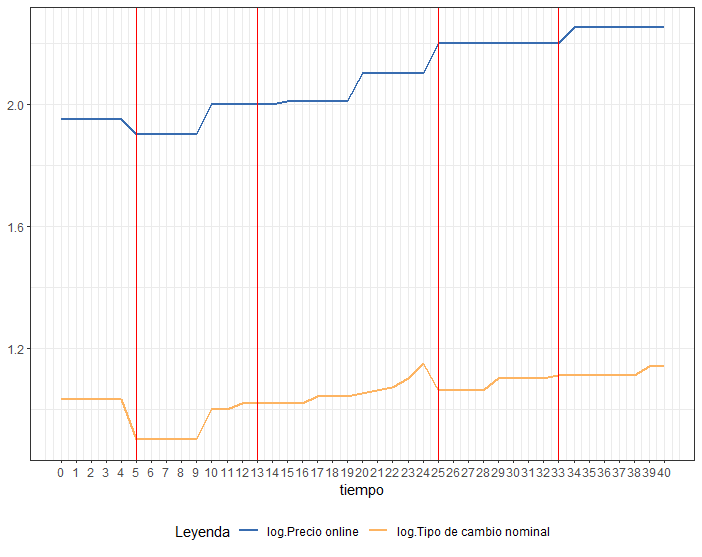
\includegraphics[scale=0.7]{metodologia.png}
  \label{fig:TIlustración de la regresión Life Long PassThrough}
\end{figure}

Por otro lado, la metodología original relaciona la frecuencia de ajuste de precios con la heterogeneidad del traspaso. En base a esa idea y a la revisión de literatura mencionada se plantea una generalización del modelo donde la heterogeneidad se explica por las características a nivel de bienes para los precios de internet.


El traspaso de larga vida se estima con la siguiente regresión generalizada a nivel de producto:
\begin{equation}
\Delta P_{it} = \beta_{0} +\beta_{1} \Delta S_{it}  + \beta_{2} \Delta S_{it}*X_{i} + \beta_{3}X_{i} + \beta_{4}Categorias + \beta_{5}Controles + \varepsilon_{it}
\end{equation}

Donde $\Delta P_{it}$ representa el cambio acumulado del precio del bien desde la primera observaci\'on del nuevo precio hasta el siguiente nuevo precio, $\Delta S_{it}$ representa el cambio acumulado del tipo de cambio desde la primera observaci\'on del nuevo precio hasta la ultima observaci\'on del nuevo precio rezagado 20 d\'ias atr\'as, $X_{i}$ es el factor que captura la heterogenidad del traspaso porque representa las características propias de los bienes. La variable dummy $Categorias$ muestra la clasificaci\'on de los productos y por último,	$Controles$ que contiene las variables duración del precio del bien y una dummy que controla por ofertas.
El comercio electronico presenta dias claves donde los precios de los productos presentan una caída y este efecto no necesariamente se explica por un apreciación cambiaria sino por dias de descuentos que afectan a todos los precios.

La heterogenidad del traspaso se captura no solo por la inclusión de la característica del bien en niveles sino también por la variable interactiva que multiplica la variación del tipo de cambio acumulado por la característica del bien.

La primera regresión que se deriva de la metodología generaliza es que el traspaso del tipo de cambio depende de la frecuencia de ajuste de precios del bien. Esta relación esta capturada por la siguiente ecuación:
\begin{equation}
\Delta P_{it} = \beta_{1} \Delta S_{it}  + \beta_{2} \Delta S_{it}*f_{i} + \beta_{3}f_{i} + \beta_{4}Categorias + \beta_{5}Controles_{i} + \varepsilon_{it}
\end{equation}
Donde $f_{i}$ cuantifica la frecuencia de ajuste de precios de cada bien.

La segunda regresión que se deriva relaciona si un precio denominado caro o barato determina el nivel del traspaso del tipo de cambio y esto se representa en la siguiente ecuación.
\begin{equation}
\Delta P_{it} = \beta_{1} \Delta S_{it}  + \beta_{2} \Delta S_{it}*P_{i} + \beta_{3}P_{i} + \beta_{4}Categorias + \beta_{5}Controles_{i} + \varepsilon_{it}
\end{equation}
Donde $P_{i}$ es el precio inicial del bien y captura el tamaño del precio.

\clearpage

%%%%%%%%%%%%%%%%%%%%%%%%%%%%%%%%%%%%%%%%%%%%%%%%%%%%%%%%%%%%%%%%%%%%%%%%%%%%%%%
\section{\underline{Resultados}}\label{sec4}

En esta sección se presentan los resultados de las estimaciones realizadas para el modelo de frecuencia de ajuste de precios y tamaño del precio.

\textbf{Life-Long PassThrough: Frecuencia del bien} \\
Los resultados de la regresión se encuentran en el cuadro 5 en el anexo. La significancia de las variables muestran que existe una heterogeneidad a nivel del traspaso y este efecto esta capturado por la interacción de la variable tipo de cambio y la frecuencia de ajuste de precios $(f* \Delta S)$. El resto de las variables como la dummy de dias de ofertas, las dummies según la clasificación del bien son significativas lo que confirma lo resaltado en la literatura.
En ese sentido, al hablar de heterogeneidad el traspaso del tipo de cambio se representa en la ecuación 12, donde el nivel del traspaso depende de únicamente de la frecuencia de ajuste de precio:\\
\emph{Traspaso del tipo de cambio:\\}
\begin{equation}
PT_{i} = \beta_{1} + \beta_{2}*f_{i}
\end{equation}
Donde $\beta_{2}$ captura la heterogenidad del traspaso y tiene el coeficiente positivo $0.082$, $\beta_{1}$ tiene el valor negativo de $-0.366$. De la ecuación 12, se puede concluir que el traspaso tiene una relación positiva con la frecuencia de ajuste de precios. Además, la frecuencia de ajuste de precios de un bien debe tener un valor por encima de 14 veces para obtener un traspaso postivo y contrario, una frecuencia menor a la media de frecuencia se obtiene un traspaso negativo.

Por otro lado, se puede calcular el efecto promedio del traspaso del tipo sobre la base de datos con el promedio de ajuste de precios. Esta variable se expresa en desvios con respecto a su media, por lo tanto $\overline f$ tiene el valor de 0. En base a este calculo se obtiene un nivel de traspaso negativo promedio, pero es necesario obtener ver la significancia de este traspaso sobre toda la serie de frecuencia de ajuste.
\begin{equation}
\beta_{1} + \beta_{2}*\overline f
\end{equation}
\begin{equation}
\beta_{1} = -0.37
\end{equation}

La figura 10 muestra la relación positiva y lineal del traspaso de tipo en el eje $y$ y la frecuencia de ajuste $f$. Los resultados son acordes a los encontrado en Gopinath y Itskhoki (2010) y la explicación teorica que esta detras de esta relación positiva se basa en el Efecto Selección.

Se ejemplifica dos situaciones una donde el precio de las tiendas retail no se ajustan continuamente y otra donde los precios tienen una alta frecuencia de los precios. En el primer caso, los precios que tiene poca frecuencia de ajuste se comportan así porque están muy cerca de su precio óptimo. Al estar muy cerca del precio optimo no tiene espacio para grandes cambios de precios por lo que el deseo de la tienda retail es tener un traspaso del tipo de cambio bajo.

En cambio, en el situación donde los precios se ajustan con más frecuencia el cambio de precio es de gran tamaño porque los precios se encuentran lejos de su precio ótimo. En ese caso la firma acepta un traspaso de tipo de cambio mucho mayor que los otros tipos de precios.
\clearpage
\begin{figure}[!h]
\centering
 \caption{Nivel de traspaso y frecuencia de ajuste de precios}
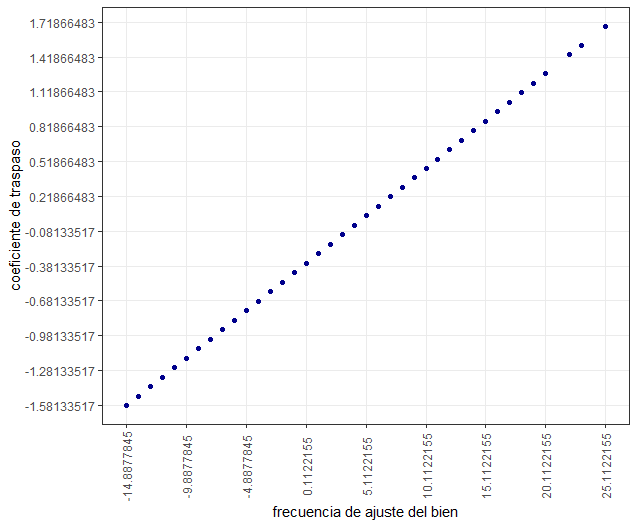
\includegraphics[scale=0.6]{E1.png}
  \label{fig:Nivel de traspaso y frecuencia de ajuste de precios}
\end{figure}

\textbf{Life-Long PassThrough: Tamaño del bien} \\
Los resultados de la regresión se encuentran en el cuadro 6 en el anexo. La significancia de las variables muestran que existe una heterogeneidad a nivel del traspaso y este efecto esta capturado por la interacción de la variable tipo de cambio y el tamaño del precio $(P* \Delta S)$. El resto de las variables como la dummy de dias de ofertas, las dummies según la clasificación del bien son significativas como en el modelo anterior. Asimismo, se estima un traspaso heterogéneo que depende lineal y positivamente del tamaño del precio. \\
Por otro lado, se puede calcular el efecto promedio del traspaso del tipo de cambio sobre la base de datos con el promedio de ajuste de precios. Se toma el promedio del precio inicial para cada bien y se obtiene que en promedio los precios de la base están 982.80 soles. En base a este cálculo se obtiene un nivel de traspaso positivo promedio, pero es necesario obtener ver la significancia de este traspaso sobre toda la serie de tamaño de precios.

Traspaso del tipo de cambio:\\
\begin{equation}
PT_{i}= \beta_{1} + \beta_{2}*P_{i}
\end{equation}
Traspaso Medio del tipo de cambio:\\
\begin{equation}
\beta_{1} + \beta_{2}*\overline P
\end{equation}
\begin{equation}
\beta_{1} + \beta_{2}*982.80 = 0.134
\end{equation}

La figura 11 muestra la relación positiva y lineal del traspaso de tipo de cambio (PT) en el eje $y$ y el tamaño de precios $P$ en el eje $x$.
\begin{figure}[!ht]
\centering
 \caption{Nivel de traspaso y tamaño del precio}
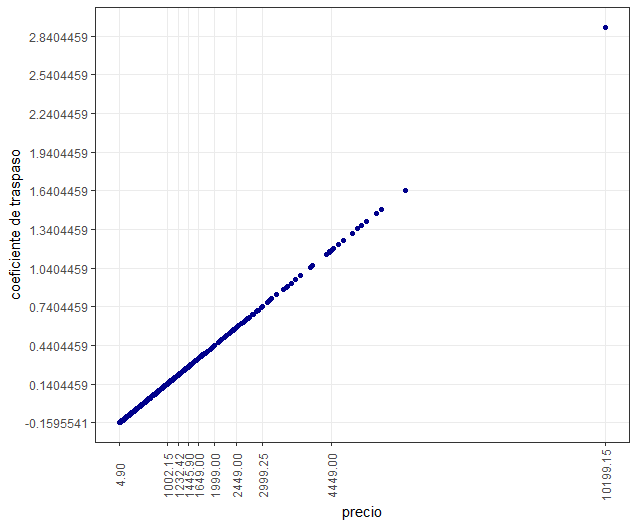
\includegraphics[scale=0.6]{E2.png}
  \label{fig:Nivel de traspaso y tamaño del precio}
\end{figure}
\clearpage
%%%%%%%%%%%%%%%%%%%%%%%%%%%%%%%%%%%%%%%%%%%%%%%%%%%%%%%%%%%%%%%%%%%%%%%%%%%%%%%%%%%%%%%%%%%%%%%%%%%%%%%%%%
\section{\underline{Conclusiones}}\label{sec5}
\begin{itemize}
	\item El traspaso del tipo de cambio aumenta conforme aumenta la frecuencia de ajuste de los precios de cada bien. Frecuencias de ajuste muy bajas puede considerarse traspaso cero.\\
	\item El traspaso del tipo de cambio aumenta conforme aumenta el costo del bien. Mientras más barato sea el bien menor traspaso se encuentra e incluso no existe traspaso. \\
\end{itemize}
\clearpage
\newpage


\bibliographystyle{chicago}
%bibliographystyle{apacite}                            % Estilo bibliográfico
\bibliography{TesisBIB}

%%%%%%%%%%%%%%%%%%%%%%%%%%%%%%%%%%%%%%%%%%%%%%%%%%%%%%%%%%%%%%%%%%%%%%%%%%%%%%%%%%%%%%%%%%%%%%%%%%%%%%%%%%
\section{\underline{Anexo}}\label{sec6}

\begin{table}[!htbp]
\caption{Estimaciones del modelo 1}\label{cor1}
\centering
\resizebox{\textwidth}{!}{\begin{tabular}{@{\extracolsep{5pt}} ccccc}
\\[-1.8ex]\hline
\hline \\[-1.8ex]
 & Estimate & Std. Error & t value & Pr(\textgreater \textbar t\textbar ) \\
\hline \\[-1.8ex]
S & $$-$0.366$ & $0.192$ & $$-$1.912$ & $0.056$ \\
S*f& $0.082$ & $0.017$ & $4.673$ & $0.00000$ \\
f& $0.0002$ & $0.0002$ & $0.746$ & $0.456$ \\
DummyOfertas& $$-$0.422$ & $0.004$ & $$-$105.771$ & $0$ \\
categoriaAudio & $0.246$ & $0.006$ & $39.680$ & $0$ \\
categoriaComputadores & $0.254$ & $0.009$ & $28.256$ & $0$ \\
categoriaElectrodomésticos & $0.240$ & $0.004$ & $59.659$ & $0$ \\
categoriaElectrohogar & $0.220$ & $0.012$ & $19.030$ & $0$ \\
categoriaFotografía & $0.282$ & $0.008$ & $35.693$ & $0$ \\
categoriaLinea blanca & $0.244$ & $0.004$ & $62.576$ & $0$ \\
categoriaTeléfonos & $0.233$ & $0.007$ & $33.414$ & $0$ \\
categoriaTelevisores & $0.240$ & $0.015$ & $16.120$ & $0$ \\
\hline \\[-1.8ex]
\end{tabular}}
\label{table:3}
\end{table}

\begin{table}[!htbp]
\caption{Estimaciones del modelo 2}\label{cor1}
\centering
\resizebox{\textwidth}{!}{\begin{tabular}{@{\extracolsep{5pt}} ccccc}
\\[-1.8ex]\hline
\hline \\[-1.8ex]
 & Estimate & Std. Error & t value & Pr(\textgreater \textbar t\textbar ) \\
\hline \\[-1.8ex]
S & $$-$0.161$ & $0.144$ & $$-$1.115$ & $0.265$ \\
S*P & $0.0003$ & $0.00001$ & $29.638$ & $0$ \\
P& $$-$0.00002$ & $0.00000$ & $$-$45.789$ & $0$ \\
DummyOferta& $$-$0.311$ & $0.004$ & $$-$83.829$ & $0$ \\
Duracion & $$-$0.0003$ & $0.00005$ & $$-$5.929$ & $0$ \\
categoriAaudio & $0.175$ & $0.005$ & $33.949$ & $0$ \\
categoriaComputadores & $0.182$ & $0.008$ & $24.218$ & $0$ \\
categoriaElectrodomésticos & $0.171$ & $0.004$ & $48.436$ & $0$ \\
categoriaElectrohogar & $0.135$ & $0.009$ & $14.763$ & $0$ \\
categoriaFotografía & $0.231$ & $0.007$ & $34.815$ & $0$ \\
categoriaLinea blanca & $0.180$ & $0.004$ & $47.033$ & $0$ \\
categoriaTeléfonos & $0.129$ & $0.010$ & $13.393$ & $0$ \\
categoriaTelevisores & $0.178$ & $0.011$ & $16.118$ & $0$ \\
\hline \\[-1.8ex]	
\end{tabular}}
\label{table:4}
\end{table}


\end{document} 